
\documentclass[12pt]{article}



\usepackage{graphicx}

\title{}

%%% BEGIN DOCUMENT
\begin{document}


\section{Component Overview}

\subsection{Configuration}
\subsection{Node Editor}

\subsection{Multi-Node Editor}
The multi-node editor component is in charge of editing all the nodes within a grid. This component handles the selection of individual or multiple nodes. For example, the user may want to select a 20x20 sub-grid and change the color to green. The multi-node editor is responsible for allowing the user to select the 400 nodes. 

This selection should be done in a way that is familiar to the user. One possible action-sequence starts with the user selecting a node in the corner of the sub-grid. Then, while holding down shift, the user would select the node in the corner of the sub-grid diagonal to the first node selected. The multi-node editor would be responsible to select all of the nodes in the sub-grid.

After nodes are selected, the multi-node editor should give the user an opportunity to edit the properties (like color or on/off status) via the single-node editor. 

The multi-node editor should also display a representation of the grid to the user via the GUI. See below for a mockup of the selection of a 2x2 sub-grid within an 8x8 grid.

\subsection{Grid Editor}
The grid editor is responsible for the creation, selection, and manipulation of grids. Since the goal of this program is to create visualizations with the nodes, it is paramount to create the functionality to create and edit multiple grids. The grids work similar to a sprite animation; there is a collection of grids that will be cycled through in real-time with a slight delay. This can be used creatively to show animations.

In regards to creation, the grid editor must take user input to create a new grid (perhaps a '+' button) and create corresponding data and GUI representations of the new grid. The user must also be able to delete grids. This component creates the ability to select single or multiple grids in a similar fashion to the multi-node editor.

Additionally, the grid editor should allow the user to rearrange grids. This could take the form of dragging an individual grid to a different location within the array of grids. Navigation of the various grids is necessary. The grid editor will implement this functionality, perhaps with a scroll bar (see figure below).

\begin{figure}[ht!]
\centering
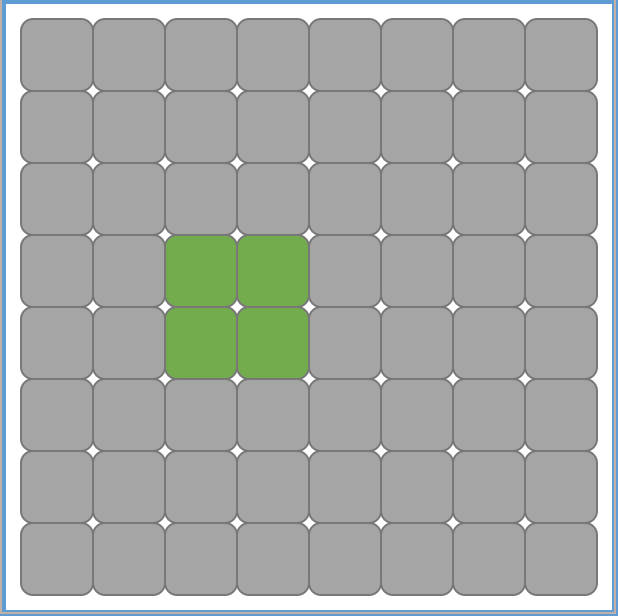
\includegraphics[width=80mm]{Grid.png}
\caption{Grid Selection (green nodes are selected)}
\end{figure}

\begin{figure}[ht!]
\centering
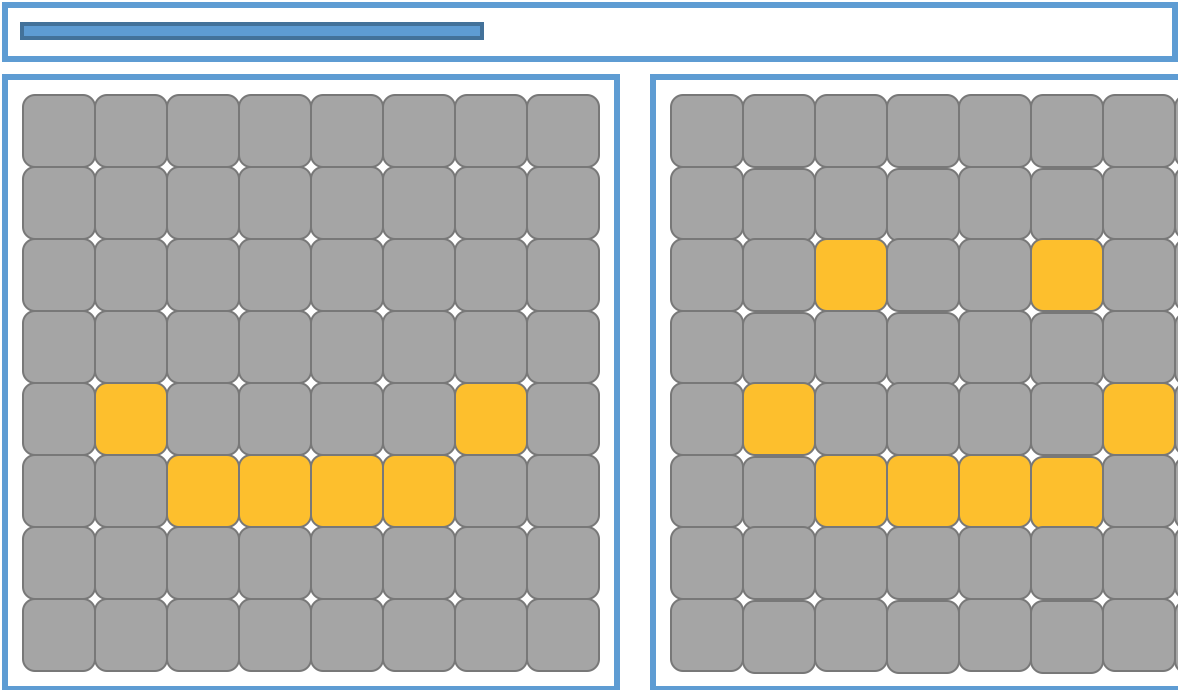
\includegraphics[width=100mm]{Multi-grid.png}
\caption{Grid Editor w/ Scroll Bar}
\end{figure}
\clearpage

\subsection{Character Editor}
The character editor is responsible for the creation, editing, and saving of special grid formations, known as characters. By default, letters and numbers (and perhaps other standard keyboard characters) should exist in the character editor. Each character, like the letter 'A', has a corresponding grid that lights up the to represent the character.

It is important to note that these default characters should be available regardless of the grid size. The character editor should allow the user to easily change the color of the character, regardless of whether it is a default character or not.

Additionally, the character editor should allow for the creation of new characters. For example, ':)' might be saved as 'smiley face'. These user-created characters are intrinsically tied to their corresponding grid size. These new characters must also be saved for future use.

\subsection{Animation Creator}
The animation creator should implement the functionality to allow the user to create animations with characters. The animation creator should supply a text box for the user to input characters. The animation editor should then allow the user to pick an animation, like scrolling left to right, for the sequence of the characters.

Based off of this, the animation creator should generate corresponding grids that simulates the animation of the characters. The user, if they so choose, should be able to edit the generated grids with the other components. 

\subsection{File Generator}
This component is responsible for outputting a text representation of the animations created in the program. The file must be in the "tan" format for use by the glasses and for future editing via this program.

\section{Component Relationships}
The first component that the user will interact with is the configuration component. Setup steps, like setting grid size, will be taken and will prepare the way for the other components to take over.

After setup, a default grid of size n by m (as specified by the user to the configuration component) should be displayed. The grid editor is responsible for creating new grids and creating a multi-node editor instances to manage every new grid. When a node is deleted via the grid editor, the grid editor is responsible to destroy the multi-node editor for the deleted grid.

When the user selects one or multiple nodes and chooses to edit their properties, the multi-node editor is responsible to call up the node editor. The node editor will then change the data representation of the edited node(s) which will then be reflected in the GUI as displayed by the multi-node editor.

Alternatively, the user can use the animation creator to generate grids which can then be edited with the grid editor, multi-node editor, and node editor. The animation editor uses characters available through the character editor.

See the use case diagram below.

\begin{figure}[ht!]
\centering
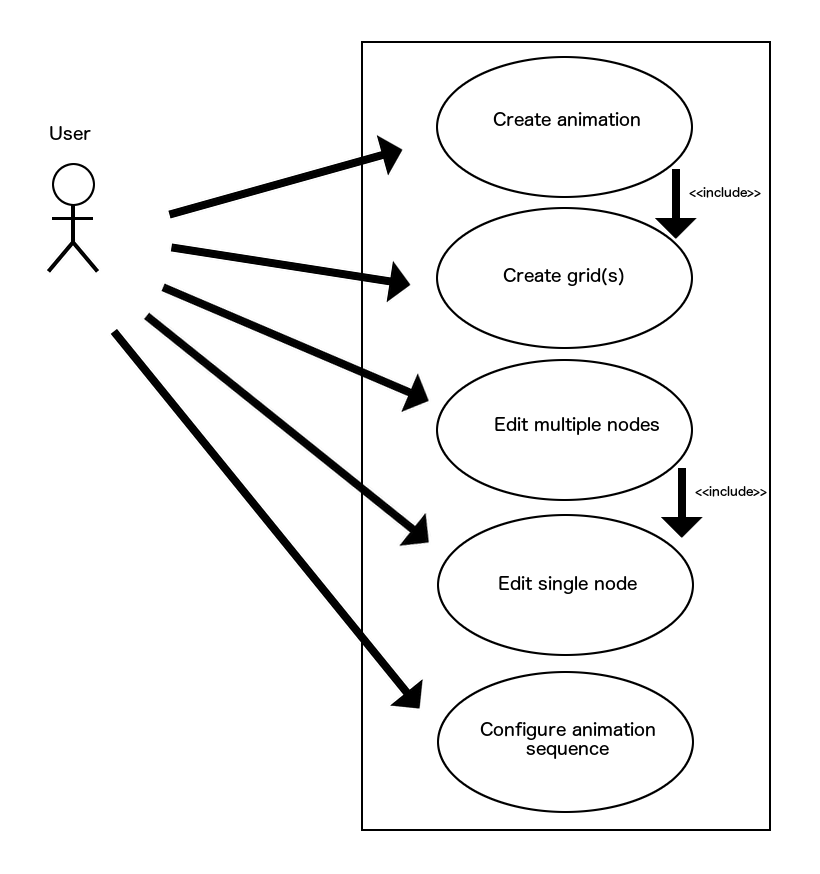
\includegraphics[width=100mm]{Relationship_Use.png}
\caption{Use Cases}
\end{figure}
\clearpage


\end{document}